\documentclass[conference]{IEEEtran}
\IEEEoverridecommandlockouts%
\usepackage{cite}
\usepackage{amsmath,amssymb,amsfonts}
\usepackage{algorithmic}
\usepackage{graphicx}
\usepackage{textcomp}
\usepackage{xcolor}
\def\BibTeX{{\rm B\kern-.05em{\sc i\kern-.025em b}\kern-.08em
    T\kern-.1667em\lower.7ex\hbox{E}\kern-.125emX}}
\begin{document}

\title{La física de transistores de película delgada con silicio amorfo}

\author{\IEEEauthorblockN{1\textsuperscript{st}MARTIN J. POWELL}
\IEEEauthorblockA{\textit{dept (of Aff.)} \\
\textit{name of organization (of Aff.)}\\
City, Country \\
email address or ORCID}}

\maketitle

\begin{abstract}
    Los transistores de película delgada de silicio amorfo son importantes
    dispositivos electrónicos que son usados en un amplio rango de aplicaciónes
    en el area de electronica. La física básica subyacente a su funcionamiento
    y los problemas clave de rendimiento se analizan aquí. Las
    características estáticas de los transistores son determinadas por la localización
    de estados electrónicos que ocurren en el bandgap de silicio amorfo.
    Los estados profundos, consisten principalmente en enlaces sueltos de
    Si, esto sirve para determinar el voltaje de umbral y determinar los estados de cola
    del bandgap en la banda de conducción y determinar la movilidad de efecto de campo. 
    Los tiempos finitos de captura y emisión de los estados
    localizados profundos conducen a una característica dinámica del transistor
    que puede describirse mediante un voltaje de umbral dependiente del
    tiempo. 
    \\
    Los transistores también muestran cambios de voltaje de umbral
    con respecto a tiempo más largos debido a otros dos mecanismos distintos; 
    a saber, la captura de carga en el aislante de compuerta de nitruro de silicio y la
    creación de estados de enlaces colgantes metaestables en el silicio amorfo. Estos
    dos mecanismos muestran características diferentes por polarización,
    temperatura, y las dependencia del cambio de voltaje de umbral. La iluminación de 
    los TFT`s causa una generación de pares electron-hueco, en la
    region de carga espacial lo que lleva a un flujo igual de estados estacionarios
    de electrones, huecos y una reducción en la flexion de la banda. En la
    mayoría de aplicaciones, la foto-sensibilidad podría ser minimizada. 
    \\
    Esto se puede hacer disminuyendo el grosor de la capa-$i$, que es más eficaz en
    los TFT`s que utilizan un aislante superior de nitruro de silicio adicional.
    La interfaz superior tiene una alta densidad de centros de recombinación,
    los cuales matan la foto-sensibilidad con una degradación minima de las
    características de transferencia. Las capas de pasivación depositadas sobre
    los TFT`s pueden afectar las características del transistor, si la capa
    de pasivación esta en contacto directo con la capa de silicio amorfo. El
    efecto consecuente sobre las características de transistores depende sobre
    el grosor de las capas. La uniformidad de arreglos grandes de transistores
    para aplicaciones de pantalla es excelente, con variaciones en el voltaje
    de umbral de 0.5 to 1.0V. El rendimiento de los dispositivos también es
    bueno, pero se necesitan más mejoras para la reducción de costes y las
    aplicaciones de mayor tamaño.
\end{abstract}

\begin{IEEEkeywords}
component, formatting, style, styling, insert
\end{IEEEkeywords}

\section{Introduccción}
    Transistores de película delgada de silicio amorfo fueron propuestos como dispositivos
    aplicables por LeComber et al. [1] en 1979. Desde entonces, ha
    habido una enorme actividad, en todo el mundo, que ha dado lugar a la utilización 
    de estos dispositivos en una variedad de aplicaciones. Quizás el mejor
    ejemplo es la matriz activa dirigido a pantallas de cristal liquido, El cual ha sido
    propuesto por mas de 20 compañías y ha liderado, en algunos casos, productos
    comerciales (para un resúmen de estas actividades se pueden ver [2]). Otras aplicaciones
    importantes incluidas de arreglos lineales de sensores de imagen para
    lectores de caras y arreglos lineales para el manejo nuevas impresoras de pagina
    amplia [4]. En todas estas aplicaciones, un minucioso entendimiento de la física
    básica subyacente la operación y el desempeño de los transistores de película
    delgada es esencial, y esto es el objetivo de este articulo. En artículos previos
    [5], el autor describe la relación del desempeño de las propiedades básicas de los
    materiales. Este articulo cubre terreno similar, concentrándose en los temas en
    los que se han producido avances desde 1984.

\section{Tecnologías TFT}
    Los transistores de película delgada de silicio amorfo puede ser hechos con una amplia
    variedad de estructuras y materiales. Básicamente, existen cuatro tipos
    de TFT`s (figura~\ref{fig1}.) Estos definidos por el orden del deposito de las capas, tales como el semiconductor,
    aislante de compuerta, contactos drenaje-fuente, y el electrodo de
    compuerta. Las estructuras escalonadas de los TFt`s tienen los contactos de fuente y drenaje
    sobre un lado del semiconductor y del electrodo de contacto sobre el lado opuesto,
    mientras las estructuras coplanar tienen los tres electrodos sobre
    el mismo lado de la película semiconductora. En la estructura ``invertida'' el
    electrodo de compuerta es la primera capa depositada sobre sustrato de vidrio.
    Los transistores de película delgada de silicio amorfo han realizado con cuatro estructuras,
    pero para todos los datos de los dispositivos usados en aplicaciones
    practicas usan una estructura escalonada. Este contraste para los TFT`s de silicio
    policristalino, los cuales son usualmente una estrcutura coplanar, que es el análogo 
    a transistores MOS de silicio cristalino.

\begin{figure}[htbp]
    \centerline{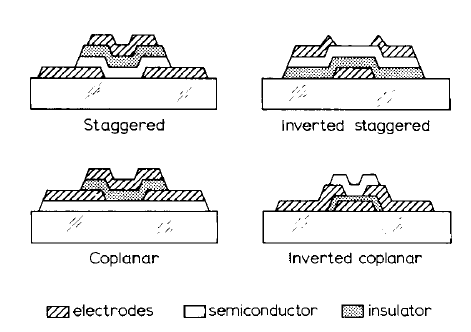
\includegraphics[width=7cm]{img/imagen-1.png}}
    \caption{Example of a figure caption.}%
    \label{fig1}
\end{figure}

    Para TFT de silicio amorfo, la estructura mas popular y una de las mas responsables
    para el estado del arte con respecto al desempeño, es el escalonado invertido, el
    cual usa nitruro de silicio como aislante de compuerta [7]. En este articulo, nos
    concentramos sobre este tipo de TFT, todos los resultados obtenidos y discutidos
    sobre este tipo de transistor. Ademas, la física de algunos tópicos es generalmente
    aplicable para algún tipo de TFT de silicio amorfo.
    \\
    Incluso limitándonos al TFT de escalonamiento invertido, hay muchas tecnologías 
    de TFT`s diferentes. La figura~\ref{fig2}, muestra dos tipos de estructuras de TFT`s
    escalonadas invertidas para silicio amorfo el cual ha sido investigado en nuestro
    laboratorio [8]. Las características más comunes de estos TFT`s son el uso de Cr como
    metal para el electrodo de compuerta, como aislante de compuerta nitruro de
    silicio, y la doble capa de metalización Cr/Al para los contactos fuente drenaje.
    La diferencia esencial es el orden de deposito de otras capas. En el tipo A
    existen TFT`s de un deposito consecutivo de nitruro de compuerta, silicio amorfo
    intrínseco, silicio amorfo $n^+$ en un solo paso de crecimiento. El $n^+$ se graba en
    la región del canal del transistor. En el caso del TFT de tipo B, existe un deposito
    consecutivo de nitruro para la compuerta, silicio amorfo intrínseco, y después
    la segunda capa de nitruro de silicio. El nitruro encima es grabado desde las
    regiones de contacto, antes de depositar la capa de $n^+$.

\begin{figure}[htbp]
    \centerline{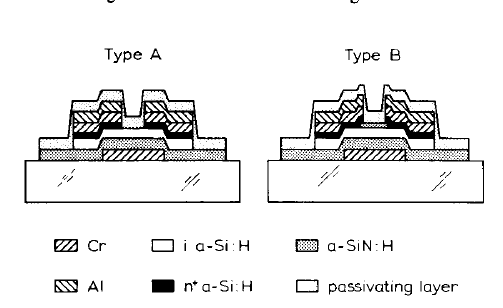
\includegraphics{img/imagen-2.png}}
    \caption{Example of a figure caption.}%
    \label{fig2}
\end{figure}

    Estos tipos de TFT`s han sido investigados por numerosos grupos. Además, todavía 
    hay diferencias en los detalles de la tecnología utilizada por cada grupo.
    Las variaciones incluyen diferentes esquemas de metalización, la posición de
    electrodo transparente, y la adición de una capa de protección ligera o un condensador
    de almacenamiento. El tipo de TFT B requiere un mínimo de tres
    pasos de mascara y el tipo B un mínimo de cuatro pasos de mascaras, pero
    algunas variaciones anteriores pueden aumentar la complejidad del proceso a
    seis o incluso ocho pasos de mascaras.










\begin{thebibliography}{00}
\bibitem{b1} G. Eason, B. Noble, and I. N. Sneddon

\end{thebibliography}


\end{document}